\subsection{Main results: performance, fairness and clustering quality}
Table~\ref{tab:main} reports all metrics on Fashion-MNIST for the ten methods. Accuracy is \emph{with} the prior correction~\eqref{eq:pc}, applied identically to every method; the uncorrected mean accuracy is shown in the first column.

\begin{table}[!htbp]
\centering
\caption{Fashion-MNIST, 40 clients, 3 seeds. Acc: mean local accuracy (with prior correction, $\pm$ std over seeds). Acc (raw): without correction. Acc@10\%: mean accuracy of the worst 10\% of clients. Worst-grp: accuracy of the worst concept group. Concept: accuracy on the class-balanced test set of the client's concept. Conflict\%: fraction of conflicting client pairs merged into one cluster (lower is better). IFCA, FeSEM, FL+HC and PACFL receive the true $K$; DisCo-CFL finds it. Oracle uses the ground-truth groups. Best non-oracle values in bold.}\label{tab:main}
\scriptsize
\setlength{\tabcolsep}{3.2pt}
\begin{tabular}{lccccccccc}
\toprule
Method & Acc (raw) & Acc & Acc@10\% & Worst-grp & Concept & Jain & ARI & K & Conflict\% \\
\midrule
\multicolumn{10}{l}{\textit{Rotation}}\\
FedAvg & 76.6 & 86.0$\pm$0.5 & 76.5 & 82.9 & 75.7 & 0.99 & 0.00 & 1.0 & 100.0 \\
Local & 87.8 & 87.8$\pm$0.7 & 80.8 & 86.9 & 60.7 & \textbf{1.00} & 0.00 & 40.0 & \textbf{0.0} \\
FedAvg-FT & 88.8 & 88.8$\pm$0.5 & 81.5 & 88.0 & 77.9 & \textbf{1.00} & 0.00 & 40.0 & \textbf{0.0} \\
IFCA & 83.5 & 89.2$\pm$1.0 & 80.9 & 86.7 & 77.0 & \textbf{1.00} & 0.41 & 4.0 & 22.0 \\
FeSEM & 83.0 & 89.1$\pm$0.3 & 80.8 & 87.8 & 80.6 & \textbf{1.00} & 0.67 & 4.0 & 10.4 \\
MTCFL & 89.4 & 90.2$\pm$0.6 & 83.6 & 89.1 & 73.9 & \textbf{1.00} & 0.15 & 34.7 & \textbf{0.0} \\
FL+HC & 78.5 & 86.4$\pm$0.4 & 76.9 & 83.6 & 74.9 & 0.99 & 0.01 & 4.0 & 85.0 \\
PACFL & 82.8 & 89.5$\pm$0.8 & 81.8 & 87.8 & 79.4 & \textbf{1.00} & 0.48 & 4.0 & 21.0 \\
DisCo & 84.5 & \textbf{90.5$\pm$0.4} & \textbf{84.6} & \textbf{89.5} & \textbf{83.9} & \textbf{1.00} & \textbf{1.00} & 4.0 & \textbf{0.0} \\
Oracle & 84.5 & 90.5$\pm$0.4 & 84.6 & 89.5 & 83.9 & 1.00 & 1.00 & 4.0 & 0.0 \\
\midrule
\multicolumn{10}{l}{\textit{Label swap}}\\
FedAvg & 54.2 & 70.1$\pm$1.4 & 47.2 & 58.6 & 55.7 & 0.94 & 0.00 & 1.0 & 100.0 \\
Local & 88.7 & 88.7$\pm$0.7 & 80.1 & 87.0 & 64.0 & \textbf{1.00} & 0.00 & 40.0 & \textbf{0.0} \\
FedAvg-FT & 90.6 & 90.6$\pm$0.5 & 84.1 & \textbf{89.7} & 80.9 & \textbf{1.00} & 0.00 & 40.0 & \textbf{0.0} \\
IFCA & 76.9 & 85.6$\pm$1.6 & 72.6 & 79.4 & 71.1 & 0.99 & 0.45 & 4.0 & 17.1 \\
FeSEM & 80.4 & 87.5$\pm$5.0 & 76.3 & 83.0 & 79.8 & 0.99 & 0.87 & 4.0 & 5.7 \\
MTCFL & 88.2 & 90.4$\pm$0.6 & 84.3 & 87.8 & 76.1 & 0.99 & 0.30 & 29.0 & 2.8 \\
FL+HC & 58.4 & 71.5$\pm$1.1 & 47.0 & 61.1 & 59.1 & 0.93 & 0.01 & 4.0 & 85.7 \\
PACFL & 57.9 & 74.8$\pm$2.6 & 50.7 & 67.8 & 53.6 & 0.94 & -0.01 & 4.0 & 34.9 \\
DisCo & 85.4 & \textbf{90.8$\pm$0.3} & \textbf{84.6} & 89.2 & \textbf{84.9} & \textbf{1.00} & \textbf{1.00} & 4.0 & \textbf{0.0} \\
Oracle & 85.4 & 90.8$\pm$0.3 & 84.6 & 89.2 & 84.9 & 1.00 & 1.00 & 4.0 & 0.0 \\
\midrule
\multicolumn{10}{l}{\textit{Rotation + QS}}\\
FedAvg & 75.9 & 85.8$\pm$0.3 & 78.4 & 82.6 & 74.7 & \textbf{1.00} & 0.00 & 1.0 & 100.0 \\
Local & 87.9 & 87.9$\pm$1.2 & 80.4 & 84.9 & 61.9 & \textbf{1.00} & 0.00 & 40.0 & \textbf{0.0} \\
FedAvg-FT & 87.6 & 87.6$\pm$0.7 & 80.8 & 84.8 & 75.4 & 0.99 & 0.00 & 40.0 & \textbf{0.0} \\
IFCA & 82.3 & 88.5$\pm$0.6 & 81.7 & 86.1 & 77.0 & \textbf{1.00} & 0.44 & 3.3 & 24.3 \\
FeSEM & 81.2 & 88.3$\pm$0.6 & 81.6 & 85.5 & 78.4 & 0.99 & 0.66 & 4.0 & 11.6 \\
MTCFL & 85.4 & 88.8$\pm$0.7 & 82.7 & 86.7 & 73.5 & \textbf{1.00} & 0.32 & 20.7 & 15.6 \\
FL+HC & 76.9 & 85.3$\pm$1.0 & 76.1 & 80.2 & 73.5 & 0.99 & 0.01 & 4.0 & 85.0 \\
PACFL & 80.1 & 88.0$\pm$1.8 & 79.7 & 84.3 & 76.5 & 0.99 & 0.44 & 4.0 & 20.8 \\
DisCo & 83.3 & \textbf{90.1$\pm$0.2} & \textbf{84.5} & \textbf{88.7} & \textbf{82.1} & \textbf{1.00} & \textbf{1.00} & 4.0 & \textbf{0.0} \\
Oracle & 83.3 & 90.1$\pm$0.2 & 84.5 & 88.7 & 82.1 & 1.00 & 1.00 & 4.0 & 0.0 \\
\bottomrule
\end{tabular}

\end{table}

\begin{table}[!htbp]
\centering
\caption*{Table~\ref{tab:main} (continued).}
\scriptsize
\setlength{\tabcolsep}{3.2pt}
\begin{tabular}{lccccccccc}
\toprule
Method & Acc (raw) & Acc & Acc@10\% & Worst-grp & Concept & Jain & ARI & K & Conflict\% \\
\midrule
\multicolumn{10}{l}{\textit{Mixed + QS}}\\
FedAvg & 70.2 & 80.8$\pm$0.9 & 66.3 & 75.1 & 66.6 & 0.98 & 0.00 & 1.0 & 100.0 \\
Local & 88.9 & 88.9$\pm$1.3 & 82.7 & 86.6 & 64.1 & \textbf{1.00} & 0.00 & 40.0 & \textbf{0.0} \\
FedAvg-FT & 88.6 & 88.6$\pm$0.9 & 82.9 & 85.7 & 76.5 & 0.99 & 0.00 & 40.0 & \textbf{0.0} \\
IFCA & 82.5 & 89.0$\pm$0.3 & 82.5 & 87.5 & 75.4 & \textbf{1.00} & 0.34 & 3.7 & 25.5 \\
FeSEM & 81.1 & 88.1$\pm$1.3 & 79.4 & 85.4 & 77.9 & 0.99 & 0.67 & 4.0 & 8.3 \\
MTCFL & 78.4 & 84.8$\pm$1.8 & 70.0 & 76.8 & 70.2 & 0.98 & 0.24 & 16.3 & 29.3 \\
FL+HC & 72.0 & 81.8$\pm$0.3 & 68.6 & 77.4 & 67.1 & 0.98 & 0.01 & 4.0 & 85.4 \\
PACFL & 71.5 & 83.3$\pm$0.4 & 68.3 & 79.3 & 66.4 & 0.98 & 0.20 & 4.0 & 21.8 \\
DisCo & 84.5 & \textbf{90.6$\pm$0.3} & \textbf{84.3} & \textbf{88.8} & \textbf{82.5} & \textbf{1.00} & \textbf{0.94} & 4.0 & 0.6 \\
Oracle & 84.2 & 90.6$\pm$0.3 & 84.6 & 88.7 & 83.4 & 1.00 & 1.00 & 4.0 & 0.0 \\
\midrule
\multicolumn{10}{l}{\textit{Label skew only}}\\
FedAvg & 87.6 & 95.5$\pm$0.4 & \textbf{90.9} & 95.5 & 85.8 & \textbf{1.00} & \textbf{1.00} & 1.0 & \textbf{0.0} \\
Local & 94.6 & 94.6$\pm$0.2 & 87.7 & 94.6 & 51.0 & \textbf{1.00} & 0.00 & 40.0 & \textbf{0.0} \\
FedAvg-FT & 94.2 & 94.2$\pm$0.3 & 90.1 & 94.2 & 80.7 & \textbf{1.00} & 0.00 & 40.0 & \textbf{0.0} \\
IFCA & 87.7 & 95.4$\pm$0.6 & 90.7 & 95.4 & 85.7 & \textbf{1.00} & \textbf{1.00} & 1.0 & \textbf{0.0} \\
FeSEM & 87.7 & 95.5$\pm$0.4 & 90.6 & 95.5 & 85.7 & \textbf{1.00} & \textbf{1.00} & 1.0 & \textbf{0.0} \\
MTCFL & 92.0 & 95.3$\pm$0.2 & 88.5 & 95.3 & 77.1 & \textbf{1.00} & 0.00 & 20.7 & \textbf{0.0} \\
FL+HC & 87.5 & 95.5$\pm$0.5 & 90.4 & 95.5 & \textbf{85.9} & \textbf{1.00} & \textbf{1.00} & 1.0 & \textbf{0.0} \\
PACFL & 87.6 & 95.5$\pm$0.4 & \textbf{90.9} & 95.5 & 85.8 & \textbf{1.00} & \textbf{1.00} & 1.0 & \textbf{0.0} \\
DisCo & 87.6 & \textbf{95.6$\pm$0.4} & 90.8 & \textbf{95.6} & 85.6 & \textbf{1.00} & 0.67 & 1.3 & \textbf{0.0} \\
Oracle & 87.6 & 95.5$\pm$0.4 & 90.9 & 95.5 & 85.8 & 1.00 & 1.00 & 1.0 & 0.0 \\
\midrule
\multicolumn{10}{l}{\textit{Minority groups}}\\
FedAvg & 77.0 & 85.5$\pm$0.7 & 74.1 & 35.7 & 76.7 & 0.98 & 0.00 & 1.0 & 100.0 \\
Local & 88.5 & 88.5$\pm$0.5 & 81.0 & 85.2 & 62.7 & \textbf{1.00} & 0.00 & 40.0 & \textbf{0.0} \\
FedAvg-FT & 89.4 & 89.4$\pm$0.5 & 82.9 & 81.7 & 78.5 & \textbf{1.00} & 0.00 & 40.0 & \textbf{0.0} \\
IFCA & 83.6 & 89.4$\pm$1.7 & 81.2 & 67.3 & 78.1 & 0.99 & 0.57 & 3.7 & 22.8 \\
FeSEM & 84.0 & 89.8$\pm$0.7 & 82.0 & 79.4 & 81.8 & \textbf{1.00} & 0.62 & 4.0 & 5.7 \\
MTCFL & 82.0 & 87.3$\pm$3.1 & 78.0 & 51.9 & 76.7 & 0.98 & 0.04 & 11.3 & 66.7 \\
FL+HC & 80.4 & 87.7$\pm$0.8 & 78.0 & 74.5 & 78.0 & 0.99 & 0.22 & 4.0 & 74.8 \\
PACFL & 83.1 & 89.8$\pm$0.7 & 83.9 & 82.7 & 78.8 & \textbf{1.00} & 0.43 & 4.0 & 17.8 \\
DisCo & 85.3 & \textbf{90.8$\pm$0.6} & \textbf{85.3} & \textbf{86.5} & \textbf{84.1} & \textbf{1.00} & \textbf{0.98} & 4.3 & \textbf{0.0} \\
Oracle & 85.3 & 90.9$\pm$0.6 & 85.3 & 86.5 & 84.2 & 1.00 & 1.00 & 4.0 & 0.0 \\
\bottomrule
\end{tabular}

\end{table}

\paragraph{DisCo-CFL recovers the concept structure without being told $K$.} In \emph{Rotation}, \emph{Label swap} and \emph{Rotation + QS}, DisCo-CFL finds exactly the ground-truth partition in all seeds (ARI $=1$) and matches the Oracle on every metric. In \emph{Mixed + QS}, where two groups differ only on 4 of the 10 classes, it reaches ARI $0.94$ with $0.6\%$ conflicting pairs merged. In \emph{Minority groups} (25/9/4/2 clients) it reaches ARI $0.98$ with no conflicts. The baselines that are given the true $K$ merge 6--86\% of the conflicting pairs: FeSEM 6--12\%, IFCA 17--26\%, PACFL 18--35\% and FL+HC 75--86\%. CFL/MTCFL has few conflicts only in the scenarios where it fragments the federation into 16--35 clusters. FL+HC groups clients by label proportions instead of concepts, PACFL by the pixel subspace (which a label swap leaves unchanged), IFCA suffers from initialisation, and FeSEM, the strongest clustering baseline, confuses nearby groups in parameter space.

\paragraph{Label skew does not create clusters.} With a single concept and strong target and quantity skew (\emph{Label skew only}), DisCo-CFL returns $K=1$ in two seeds. In the third it isolates one client whose signature for one class disagrees with all others, and flags it as \emph{anomalous} in the audit log. Accuracy equals FedAvg's. CFL/MTCFL, in contrast, splits the federation into about 20 clusters, and its concept accuracy drops from 85.8\% to 77.1\%.

\paragraph{Performance.} With the prior correction, DisCo-CFL has the best mean accuracy in every Fashion-MNIST scenario. Personalising and fragmenting methods (Local, FedAvg-FT, MTCFL with 16--35 clusters) obtain competitive \emph{local} accuracy, because local test sets share the client's skewed label mix. In the concept-shift scenarios their \emph{concept} accuracy is 4--23 points lower: their models do not generalise to the rest of the client's concept, e.g.\ to classes whose frequency will change. DisCo-CFL is best on concept accuracy in every concept-shift scenario (82.1--84.9\%, against at most 81.8\% for any baseline). The prior correction adds 5--17 points to every method that shares models across clients. It is what makes concept-level clustering competitive on local metrics, as Proposition~\ref{prop:pc} predicts.

\paragraph{Fairness.} DisCo-CFL has the best accuracy on the worst 10\% of clients in every scenario with concept shift, and the best worst-group accuracy in all of them except \emph{Label swap}, where FedAvg-FT is 0.5 points higher (89.7\% vs.\ 89.2\%). The gap is largest for minority concepts. In \emph{Minority groups}, the worst concept group reaches 86.5\% with DisCo-CFL, against 35.7\% with FedAvg, 51.9\% with MTCFL, 67.3\% with IFCA, 74.5\% with FL+HC and 79.4\% with FeSEM: the size-independence of Corollary~\ref{cor:sc} in practice. Table~\ref{tab:minority} isolates the clustering step. DisCo-CFL recovers minority groups of 1, 2, 3 and 5 clients with recall and purity $1.00$ and no conflicting merges. FL+HC isolates the minority only by spending its fixed $K$ on it while merging 81\% of the conflicting pairs among the majority groups, and PACFL does not find the minority at all.

\begin{table}[!htbp]
\centering
\caption{Minority-group recovery (clustering step only; groups of 20/10/10/$m$ clients; 3 seeds).}\label{tab:minority}
\small
\begin{tabular}{lcccccc}
\toprule
& \multicolumn{3}{c}{DisCo-CFL} & \multicolumn{3}{c}{FL+HC ($K$ given)} \\
\cmidrule(lr){2-4}\cmidrule(lr){5-7}
$m$ & recall & ARI & conflict\% & recall & ARI & conflict\% \\
\midrule
1 & 1.00 & 0.98 & 0.0 & 1.00 & 0.09 & 81.5\\
2 & 1.00 & 0.98 & 0.0 & 1.00 & 0.11 & 81.0\\
3 & 1.00 & 1.00 & 0.0 & 1.00 & 0.12 & 80.6\\
5 & 1.00 & 0.98 & 0.0 & 0.60 & 0.09 & 82.9\\
\bottomrule
\end{tabular}
\end{table}

\subsection{Other datasets}
Table~\ref{tab:other} repeats the two basic concept-shift scenarios on MNIST and CIFAR-10 with the same hyperparameters. On MNIST, DisCo-CFL again matches the Oracle: 98.5\% (rotation) and 98.7\% (label swap), with no conflicting merges. Its concept accuracy is 97--98\%, against at most 91.6\% for any baseline. In the MNIST rotation scenario two seeds leave one or two clients in singleton clusters (flagged as anomalous; mean ARI $0.97$, $K=5.0$); these clients train alone, and the mean accuracy still equals the Oracle's.

CIFAR-10 is harder, and here DisCo-CFL is not the best method on every metric. With the default 10 warm-up rounds, the reference model is only about 40\% accurate. Its class-conditional gradients hardly depend on the orientation of most natural-image classes (mean between-group similarity 0.83--0.90; only vehicle classes separate clearly). The separation $\Delta$ of Assumption~\ref{ass:sep} is then small, and DisCo-CFL reaches only ARI $0.38$, although its concept accuracy (41.0\%) is already the best among the baselines. The theory points to the remedy, a more informative reference model. With 30 warm-up rounds (DisCo-T30; the reference accuracy stays near 39\%, but orientation-sensitive features emerge), ARI rises to $0.74$, conflicting merges drop from 24.6\% to 4.2\%, and concept accuracy reaches 44.8\%, the best of all non-oracle methods. Table~\ref{tab:warm} gives the clustering-only trend. CFL/MTCFL has the highest \emph{local} accuracy on CIFAR-10 (67.0\%, above the Oracle's 64.2\%). It splits the federation into 35 clusters, i.e.\ it personalises to each client's label mix with the small CNN, and its concept accuracy is the lowest of the clustered methods (38.2\%).

\begin{table}[t]
\centering
\caption{CIFAR-10 rotation, clustering step only: effect of the warm-up length $T_0$ (3 seeds).}\label{tab:warm}
\small
\begin{tabular}{lccc}
\toprule
$T_0$ & ARI & $K$ & conflict\% \\
\midrule
10 & 0.37 & 3.7 & 24.8 \\
20 & 0.64 & 5.0 & 8.9 \\
30 & 0.74 & 4.7 & 4.2 \\
\bottomrule
\end{tabular}
\end{table}

\begin{table}[t]
\centering
\caption{MNIST and CIFAR-10 (40 clients, 3 seeds, same settings and columns as Table~\ref{tab:main}).}\label{tab:other}
\scriptsize
\setlength{\tabcolsep}{3.2pt}
\begin{tabular}{lccccccccc}
\toprule
Method & Acc (raw) & Acc & Acc@10\% & Worst-grp & Concept & Jain & ARI & K & Conflict\% \\
\midrule

\bottomrule
\end{tabular}

\end{table}

\paragraph{Robustness sweeps.}\label{sec:sweeps}
Table~\ref{tab:sweeps} varies one factor at a time on Fashion-MNIST: the strength of the concept shift, the number of groups, the fraction of participating clients and the number of clients. Baselines are given the true $K$ where they need it.

\begin{table}[!htbp]
\centering
\caption{Robustness sweeps (Fashion-MNIST, 3 seeds). For DisCo-CFL: ARI, number of clusters, conflict-merge rate, accuracy and concept accuracy. For comparison: the best baseline on accuracy and on concept accuracy (in parentheses), and the Oracle's accuracy.}\label{tab:sweeps}
\scriptsize
\setlength{\tabcolsep}{3pt}
\resizebox{\textwidth}{!}{%
\begin{tabular}{llcccccccc}
\toprule
& & \multicolumn{5}{c}{DisCo-CFL} & & & \\
\cmidrule(lr){3-7}
Factor & Setting & ARI & $K$ & Conflict\% & Acc & Concept & Best baseline Acc & Best baseline Concept & Oracle Acc \\
\midrule
Strength & $\theta=15^\circ$ & 0.42 & 3.0 & 32.1 & 90.0 & 82.8 & 90.2 (FeSEM) & 83.0 (FeSEM) & 90.5 \\
Strength & $\theta=30^\circ$ & 0.93 & 4.3 & 1.7 & 90.3 & 83.1 & 90.0 (PACFL) & 81.2 (PACFL) & 90.4 \\
Strength & $\theta=45^\circ$ & 1.00 & 4.0 & 0.0 & 90.4 & 83.8 & 89.9 (FeSEM) & 81.8 (FeSEM) & 90.4 \\
Strength & $\theta=90^\circ$ & 1.00 & 4.0 & 0.0 & 90.5 & 83.9 & 90.2 (MTCFL) & 80.6 (FeSEM) & 90.5 \\
Groups & $K=2$ & 0.94 & 3.3 & 0.0 & 91.4 & 86.5 & 88.5 (IFCA) & 80.2 (IFCA) & 91.5 \\
Groups & $K=4$ & 1.00 & 4.0 & 0.0 & 90.8 & 84.9 & 90.6 (FedAvg-FT) & 80.9 (FedAvg-FT) & 90.8 \\
Groups & $K=8$ & 0.92 & 8.0 & 0.3 & 90.4 & 81.7 & 88.0 (FeSEM) & 75.4 (FeSEM) & 90.5 \\
Participation 30\% & rotation & 1.00 & 4.0 & 0.0 & 89.1 & 78.4 & 87.5 (PACFL) & 75.1 (FeSEM) & 89.1 \\
Participation 30\% & label swap & 0.98 & 4.0 & 0.0 & 89.3 & 78.3 & 86.5 (FeSEM) & 73.0 (FeSEM) & 89.3 \\
Scale & $N=200$ & 0.98 & 6.3 & 0.0 & 91.1 & 86.6 & 89.8 (PACFL) & 83.9 (FeSEM) & 91.1 \\
\bottomrule
\end{tabular}}

\end{table}

\paragraph{Strength of the shift.} With rotations of $0,\theta,2\theta,3\theta$ degrees, DisCo-CFL separates the groups perfectly from $\theta=45^\circ$ on and almost perfectly at $30^\circ$ (ARI $0.93$). At $15^\circ$ neighbouring concepts are so close that their class-conditional gradients agree above the threshold, and DisCo-CFL merges them (ARI $0.42$). This is the behaviour predicted by the separation assumption: the method groups what it cannot tell apart. It costs little, because nearby concepts can share a model: accuracy is 90.0\% against 90.5\% for the Oracle, and 0.2 points below FeSEM, which is given $K=4$. For every $\theta\ge30^\circ$, DisCo-CFL has the best accuracy and concept accuracy and is within $0.1$ points of the Oracle.

\paragraph{Number of groups.} With $K=2$, $4$ and $8$ label-permutation groups, DisCo-CFL finds $K$ without being told (3.3, 4.0 and 8.0 clusters; the extra cluster at $K=2$ is a conflict-free split) and merges at most 0.3\% of conflicting pairs. Its accuracy is within $0.1$ points of the Oracle for all $K$. The margin over the best baseline is 2.9, 0.2 and 2.4 points in accuracy and 6.3, 4.0 and 6.3 points in concept accuracy for $K=2,4,8$. With $K=2$ and $K=8$ the baselines given $K$ confuse groups (IFCA and FeSEM merge 25\% and 4\% of the conflicting pairs), whereas with $K=4$ the fine-tuned global model is a strong competitor on local accuracy only.

\paragraph{Partial participation.} When only 30\% of the clients take part in each round, the warm-up model is noisier. DisCo-CFL still recovers the groups (ARI $1.00$ and $0.98$) and matches the Oracle, while the best baseline is 1.6--2.8 points below in accuracy and 3.3--5.3 points below in concept accuracy.

\paragraph{Number of clients.} With 200 clients of 200 samples each, DisCo-CFL reaches ARI $0.98$ with no conflicting merge. The extra clusters ($K=5$--$7$) are conflict-free splits of groups; three of them are singletons flagged as anomalous in the audit log. Accuracy equals the Oracle's (91.1\%), 1.3 points above the best baseline, and concept accuracy is 2.7 points above the best baseline. This is in line with the clustering-only scalability study of Section~\ref{sec:cost}.

\paragraph{Statistical significance.}
Table~\ref{tab:signif} compares DisCo-CFL with each baseline over all (scenario, seed) pairs with concept shift that both methods were run on. DisCo-CFL is significantly better than every baseline on mean accuracy, concept accuracy and worst-group accuracy (one-sided Wilcoxon signed-rank tests, all $p<0.01$). The closest competitors are FeSEM, MTCFL and FedAvg-FT. MTCFL and FedAvg-FT win on local accuracy mainly on CIFAR-10 (5--6 of the 6 CIFAR-10 pairs), and FeSEM wins on 8 of 57 pairs, mostly CIFAR-10 rotation and the $15^\circ$ rotation. On concept accuracy DisCo-CFL wins against every baseline in at least 84\% of the pairs.

\begin{table}[!htbp]
\centering
\caption{Paired one-sided Wilcoxon signed-rank tests of DisCo-CFL against each baseline over all (scenario, seed) pairs with concept shift. W/T/L: wins, ties ($|\Delta|<0.05$ points) and losses of DisCo-CFL.}\label{tab:signif}
\small
\begin{tabular}{lccccccc}
\toprule
& & \multicolumn{2}{c}{Accuracy} & \multicolumn{2}{c}{Concept accuracy} & \multicolumn{2}{c}{Worst-group accuracy} \\
\cmidrule(lr){3-4}\cmidrule(lr){5-6}\cmidrule(lr){7-8}
Baseline & pairs & W/T/L & $p$ & W/T/L & $p$ & W/T/L & $p$ \\
\midrule
FedAvg & 57 & 57/0/0 & 2.6e-11 & 57/0/0 & 2.6e-11 & 57/0/0 & 2.6e-11 \\
Local & 33 & 33/0/0 & 1.2e-10 & 33/0/0 & 1.2e-10 & 32/0/1 & 2.3e-10 \\
FedAvg-FT & 33 & 27/1/5 & 2.3e-5 & 33/0/0 & 1.2e-10 & 24/0/9 & 0.004 \\
IFCA & 54 & 54/0/0 & 8.1e-11 & 54/0/0 & 8.1e-11 & 54/0/0 & 8.1e-11 \\
FeSEM & 57 & 45/4/8 & 2.5e-8 & 48/2/7 & 1.4e-8 & 47/3/7 & 5.2e-8 \\
MTCFL & 39 & 30/2/7 & 0.002 & 39/0/0 & 1.8e-12 & 30/0/9 & 1.4e-4 \\
FL+HC & 57 & 57/0/0 & 2.6e-11 & 57/0/0 & 2.6e-11 & 57/0/0 & 2.6e-11 \\
PACFL & 57 & 54/0/3 & 7.0e-11 & 57/0/0 & 2.6e-11 & 53/1/3 & 5.1e-11 \\
\bottomrule
\end{tabular}

\end{table}


\subsection{Transparency: explanations and diagnosis}
Table~\ref{tab:fat} evaluates the class-level explanations against the ground truth. For label-swap groups, the divergent classes reported by the server are \emph{exactly} the swapped classes in every pair (precision, recall and exact match $1.00$), and the diagnosis ``class-specific concept shift'' is always correct. A typical explanation reads: \emph{``cluster 0 vs.\ cluster 2: class-specific concept shift on classes [4, 5, 6, 7]''}. Here group 2 swaps $4\leftrightarrow5$ and $6\leftrightarrow7$. For rotations, precision is $1.00$, i.e.\ no class is ever wrongly reported as divergent. Recall is $0.93$: every miss occurs between $0^\circ$ and $180^\circ$ groups, on trouser, pullover, dress and shirt, items that are nearly invariant under a $180^\circ$ rotation. For these classes the two concepts \emph{are} statistically close, so the reported ``class-specific shift'' matches the data (Proposition~\ref{prop:expl}); it only disagrees with our coarse ground-truth label ``global''.

\begin{table}[!htbp]
\centering
\caption{Transparency and accountability (Fashion-MNIST, 3 seeds, default settings).}\label{tab:fat}
\small
\begin{tabular}{lccc}
\toprule
& Rotation & Label swap & Mixed + QS \\
\midrule
\multicolumn{4}{l}{\emph{Explanations: divergent classes between clusters}}\\
precision & 1.00 & 1.00 & 1.00 \\
recall & 0.93 & 1.00 & 0.92 \\
exact set / diagnosis correct & 0.67 & 1.00 & 0.39 \\
\midrule
\multicolumn{4}{l}{\emph{Certificates}}\\
share of confident certificates & 0.95 & 0.97 & 0.93 \\
conflict-free among confident & 1.000 & 1.000 & 0.919 \\
conflict-free among uncertain & 1.000 & 1.000 & 0.778 \\
\midrule
\multicolumn{4}{l}{\emph{Newcomers}}\\
known concept, correctly assigned & 1.00 & 0.96 & -- \\
novel concept, flagged as novel & 1.00 & 1.00 & -- \\
\bottomrule
\end{tabular}
\end{table}

\subsection{Accountability: certificates, audit log, newcomers}
Certificates are informative (Table~\ref{tab:fat}). In the hardest scenario (\emph{Mixed + QS}), 91.9\% of the clients with a \emph{confident} certificate are in a conflict-free position, against 77.8\% of those with an \emph{uncertain} one. In the other scenarios all clients are correctly placed and 95--97\% receive confident certificates. The uncertain ones carry the bottleneck class that makes them ambiguous, which is what a client needs in order to contest its assignment. Newcomers that join after clustering, using the frozen reference model, are assigned to the right cluster in 96--100\% of cases. Clients with a labelling never seen during clustering are reported as a \emph{novel concept} in 100\% of cases instead of being forced into an existing cluster.

\subsection{Privacy}\label{sec:privacy-exp}
Figure~\ref{fig:dp} shows the ARI of the clustering when the signatures are released with the Gaussian mechanism of Proposition~\ref{prop:dp} ($C_{\rm clip}=0.5$, $\delta=10^{-5}$). As predicted by Proposition~\ref{prop:dp}(iii), the \emph{raw} cosine collapses to ARI $\approx0$ at every noise level: DP noise attenuates all similarities and every client looks unrelated to every other. With disattenuation, the clustering degrades gracefully, and more data per client buys more privacy, as predicted by the $h\propto\sigma_{\rm dp}$ term. With 1{,}500 samples per client, DisCo-CFL keeps ARI $0.92$ (rotation) and $0.77$ (label swap) at $\varepsilon=4.4$, and $0.68/0.60$ at $\varepsilon=2$.

\begin{figure}[!htbp]
\centering
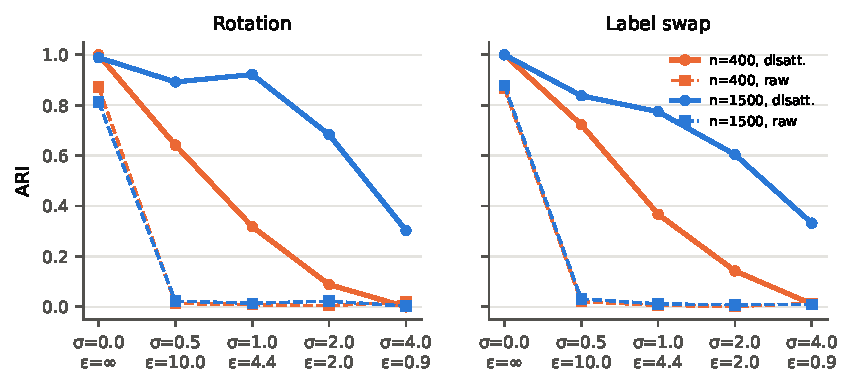
\includegraphics[width=0.85\linewidth]{../results/figures/dp.pdf}
\caption{Clustering quality under $(\varepsilon,10^{-5})$-DP signatures. Solid: DisCo-CFL; dashed: raw cosine. Orange: 400 samples per client; blue: 1{,}500.}\label{fig:dp}
\end{figure}

\subsection{Calibration and sensitivity}\label{sec:sens}
\paragraph{Calibration across sample sizes.} Varying the client size from 50 to 800 samples (Figure~\ref{fig:size} in Appendix~\ref{app:figs}), the mean disattenuated similarity between clients of the same group stays at $0.98$--$0.99$, whereas the raw cosine stays around $0.91$--$0.95$ and depends on the per-class sample counts. ARI reaches $1.00$ from 200 samples per client on (rotation) and from 400 (label swap).
\paragraph{Threshold and shrinkage.} Figure~\ref{fig:tau} shows that DisCo-CFL is stable for $\tau\in[0.75,0.85]$ in all concept-shift scenarios (ARI $0.85$--$1.00$). With the raw cosine, every $\tau$ above $0.7$ causes over-splitting ($K$ up to 16 at $\tau=0.9$). The label-only scenario is the most sensitive: $\tau\le0.7$ gives $K=1$ in all seeds, and at $\tau=0.8$ one seed flags a single anomalous client. The shrinkage $\lambda$ has almost no effect between $0.02$ and $1$ (Appendix~\ref{app:figs}), including values that satisfy the condition of Corollary~\ref{cor:sc}.

\begin{figure}[!htbp]
\centering
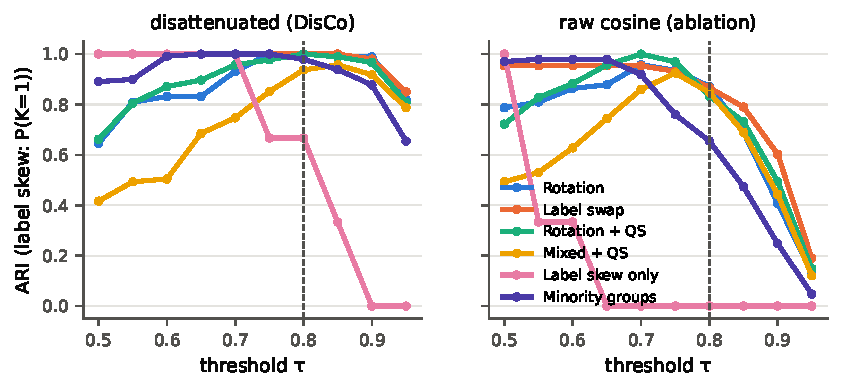
\includegraphics[width=0.85\linewidth]{../results/figures/tau_sensitivity.pdf}
\caption{Sensitivity to the threshold $\tau$ (3 seeds). The dashed line marks the default $\tau=0.8$, which was fixed before these runs.}\label{fig:tau}
\end{figure}

\subsection{Theory in practice}
Figure~\ref{fig:theory} validates the theory on synthetic signatures with known ground truth ($p=512$, noise of effective rank 16). The disattenuated similarity is nearly unbiased for every half size $h$, whereas the raw cosine is biased by up to $-0.37$. Safety and maximality are reached with probability 1 once $h\ge64$ for all separations $\Delta\in[0.2,0.7]$, and exact recovery is reached under full class support. The required $h$ grows as $\Delta$ shrinks. Recovery of a minority group of 1, 2, 4 or 8 clients follows the same curve (Figure~\ref{fig:thminority} in Appendix~\ref{app:figs}), as Corollary~\ref{cor:sc} states.

\begin{figure}[!htbp]
\centering
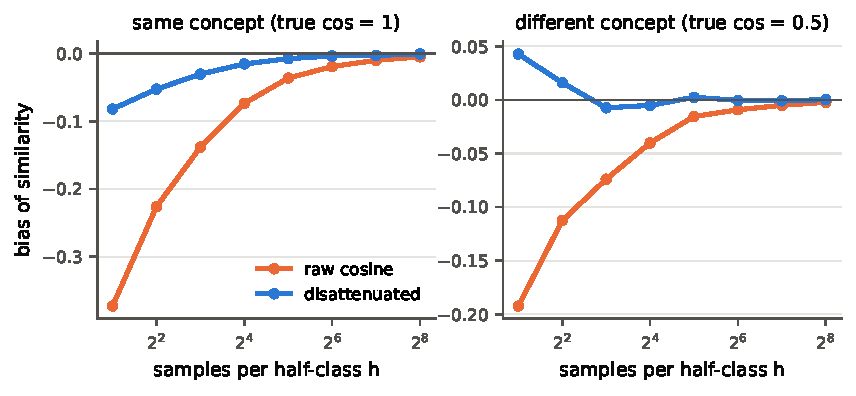
\includegraphics[width=0.49\linewidth]{../results/figures/theory_estimation.pdf}\hfill
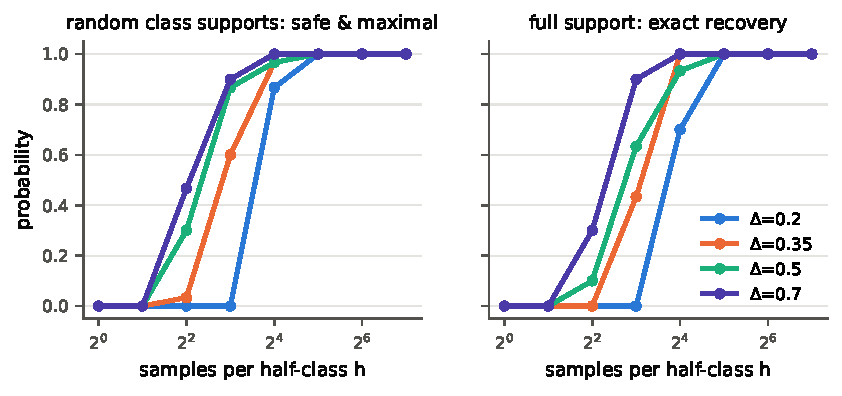
\includegraphics[width=0.49\linewidth]{../results/figures/theory_recovery.pdf}
\caption{Synthetic validation. Left: bias of the similarity estimate. Right: probability of the guarantees of Theorem~\ref{thm:rec}.}\label{fig:theory}
\end{figure}

\subsection{Ablation}
Table~\ref{tab:abl} removes one component at a time. Every component contributes. Without class conditioning (one signature per client over all its data), clients are grouped by their label mix, exactly the failure mode reported in the survey~\citep{benali2026survey}: 13--23 clusters and a concept accuracy 10--12 points lower. Without disattenuation, noise-attenuated similarities fall below the threshold and the federation is over-split, including the label-only case. The mean linkage averages class-specific shifts away and merges conflicting clients (up to 6.9\% in \emph{Mixed + QS}). Linkage-ordered merging creates bridges through ambiguous clients and over-splits. Without clipping, heavy-tailed per-sample gradients inflate the number of clusters.
\begin{table}[t]
\centering
\caption{Ablation (Fashion-MNIST, 3 seeds): ARI / number of clusters $K$ per scenario, mean conflict-merge rate and mean concept accuracy over the five scenarios.}\label{tab:abl}
\scriptsize
\setlength{\tabcolsep}{3pt}
\begin{tabular}{lccccccc}
\toprule
Variant & Rotation & Label swap & Rot.\,+\,QS & Mixed\,+\,QS & Label only & Conflict\% & Concept \\
\midrule
DisCo-CFL (full) & 1.00 / 4.0 & 1.00 / 4.0 & 1.00 / 4.0 & 0.94 / 4.0 & 0.67 / 1.3 & 0.1 & 83.8 \\
without disattenuation (raw cosine) & 0.87 / 6.7 & 0.87 / 6.0 & 0.83 / 7.0 & 0.85 / 5.7 & 0.00 / 4.0 & 0.0 & 82.4 \\
without class conditioning & 0.15 / 23.3 & 0.15 / 17.7 & 0.16 / 22.3 & 0.09 / 22.3 & 0.00 / 13.0 & 0.9 & 72.7 \\
mean instead of bottleneck linkage & 1.00 / 4.0 & 0.80 / 4.0 & 0.92 / 4.0 & 0.69 / 4.0 & 1.00 / 1.0 & 2.6 & 82.1 \\
linkage-ordered merging & 0.95 / 5.0 & 0.86 / 5.7 & 1.00 / 4.0 & 0.81 / 5.7 & 0.33 / 1.7 & 0.0 & 82.5 \\
without per-sample clipping & 0.94 / 5.0 & 1.00 / 4.0 & 0.91 / 5.7 & 0.88 / 5.3 & 0.00 / 3.0 & 0.3 & 83.0 \\
\bottomrule
\end{tabular}
\end{table}
\subsection{Other datasets}
Table~\ref{tab:other} repeats the two basic concept-shift scenarios on MNIST and CIFAR-10 with the same hyperparameters. On MNIST, DisCo-CFL again matches the Oracle: 98.5\% (rotation) and 98.7\% (label swap), with no conflicting merges. Its concept accuracy is 97--98\%, against at most 91.6\% for any baseline. In the MNIST rotation scenario two seeds leave one or two clients in singleton clusters (flagged as anomalous; mean ARI $0.97$, $K=5.0$); these clients train alone, and the mean accuracy still equals the Oracle's.

CIFAR-10 is harder, and here DisCo-CFL is not the best method on every metric. With the default 10 warm-up rounds, the reference model is only about 40\% accurate. Its class-conditional gradients hardly depend on the orientation of most natural-image classes (mean between-group similarity 0.83--0.90; only vehicle classes separate clearly). The separation $\Delta$ of Assumption~\ref{ass:sep} is then small, and DisCo-CFL reaches only ARI $0.38$, although its concept accuracy (41.0\%) is already the best among the baselines. The theory points to the remedy, a more informative reference model. With 30 warm-up rounds (DisCo-T30; the reference accuracy stays near 39\%, but orientation-sensitive features emerge), ARI rises to $0.74$, conflicting merges drop from 24.6\% to 4.2\%, and concept accuracy reaches 44.8\%, the best of all non-oracle methods. Table~\ref{tab:warm} gives the clustering-only trend. CFL/MTCFL has the highest \emph{local} accuracy on CIFAR-10 (67.0\%, above the Oracle's 64.2\%). It splits the federation into 35 clusters, i.e.\ it personalises to each client's label mix with the small CNN, and its concept accuracy is the lowest of the clustered methods (38.2\%).

\begin{table}[t]
\centering
\caption{CIFAR-10 rotation, clustering step only: effect of the warm-up length $T_0$ (3 seeds).}\label{tab:warm}
\small
\begin{tabular}{lccc}
\toprule
$T_0$ & ARI & $K$ & conflict\% \\
\midrule
10 & 0.37 & 3.7 & 24.8 \\
20 & 0.64 & 5.0 & 8.9 \\
30 & 0.74 & 4.7 & 4.2 \\
\bottomrule
\end{tabular}
\end{table}

\begin{table}[t]
\centering
\caption{MNIST and CIFAR-10 (40 clients, 3 seeds, same settings and columns as Table~\ref{tab:main}).}\label{tab:other}
\scriptsize
\setlength{\tabcolsep}{3.2pt}
\begin{tabular}{lccccccccc}
\toprule
Method & Acc (raw) & Acc & Acc@10\% & Worst-grp & Concept & Jain & ARI & K & Conflict\% \\
\midrule

\bottomrule
\end{tabular}

\end{table}



\subsection{Cost and scalability}\label{sec:cost}
Each client uploads its signature \emph{once}, about $1.2\times10^4$ floats with $p=1024$. The size is independent of the model dimension $d$; IFCA, by contrast, downloads $K$ models per client in \emph{every} round, and CFL/FL+HC cluster $d$-dimensional updates. Computing the signature takes 0.14--0.16\,s per client on one CPU core. Server-side clustering takes 0.05\,s for 40 clients and 2.3\,s for 320 clients, with ARI $\ge0.98$ at every scale.
